\section{Oscillatorer}
\textbf{HAREC a.\ref{HAREC.a.3.6}\label{myHAREC.a.3.6}}
\index{oscillator}
\label{oscillatorer}

\subsection{Alstring av svängningar}
Ordet \emph{oscillare} (lat.) har betydelsen svänga och den företeelse
eller anordning som skapar en svängning kallas oscillator.
Vid alla slags svängningar sker växelverkan mellan olika energiformer.
Svängningar förekommer i olika former.
Det kan till exempel vara vibrationer i en kropp, molekylrörelser i gaser och
vätskor eller elektriska laddningars rörelser.

\begin{figure}
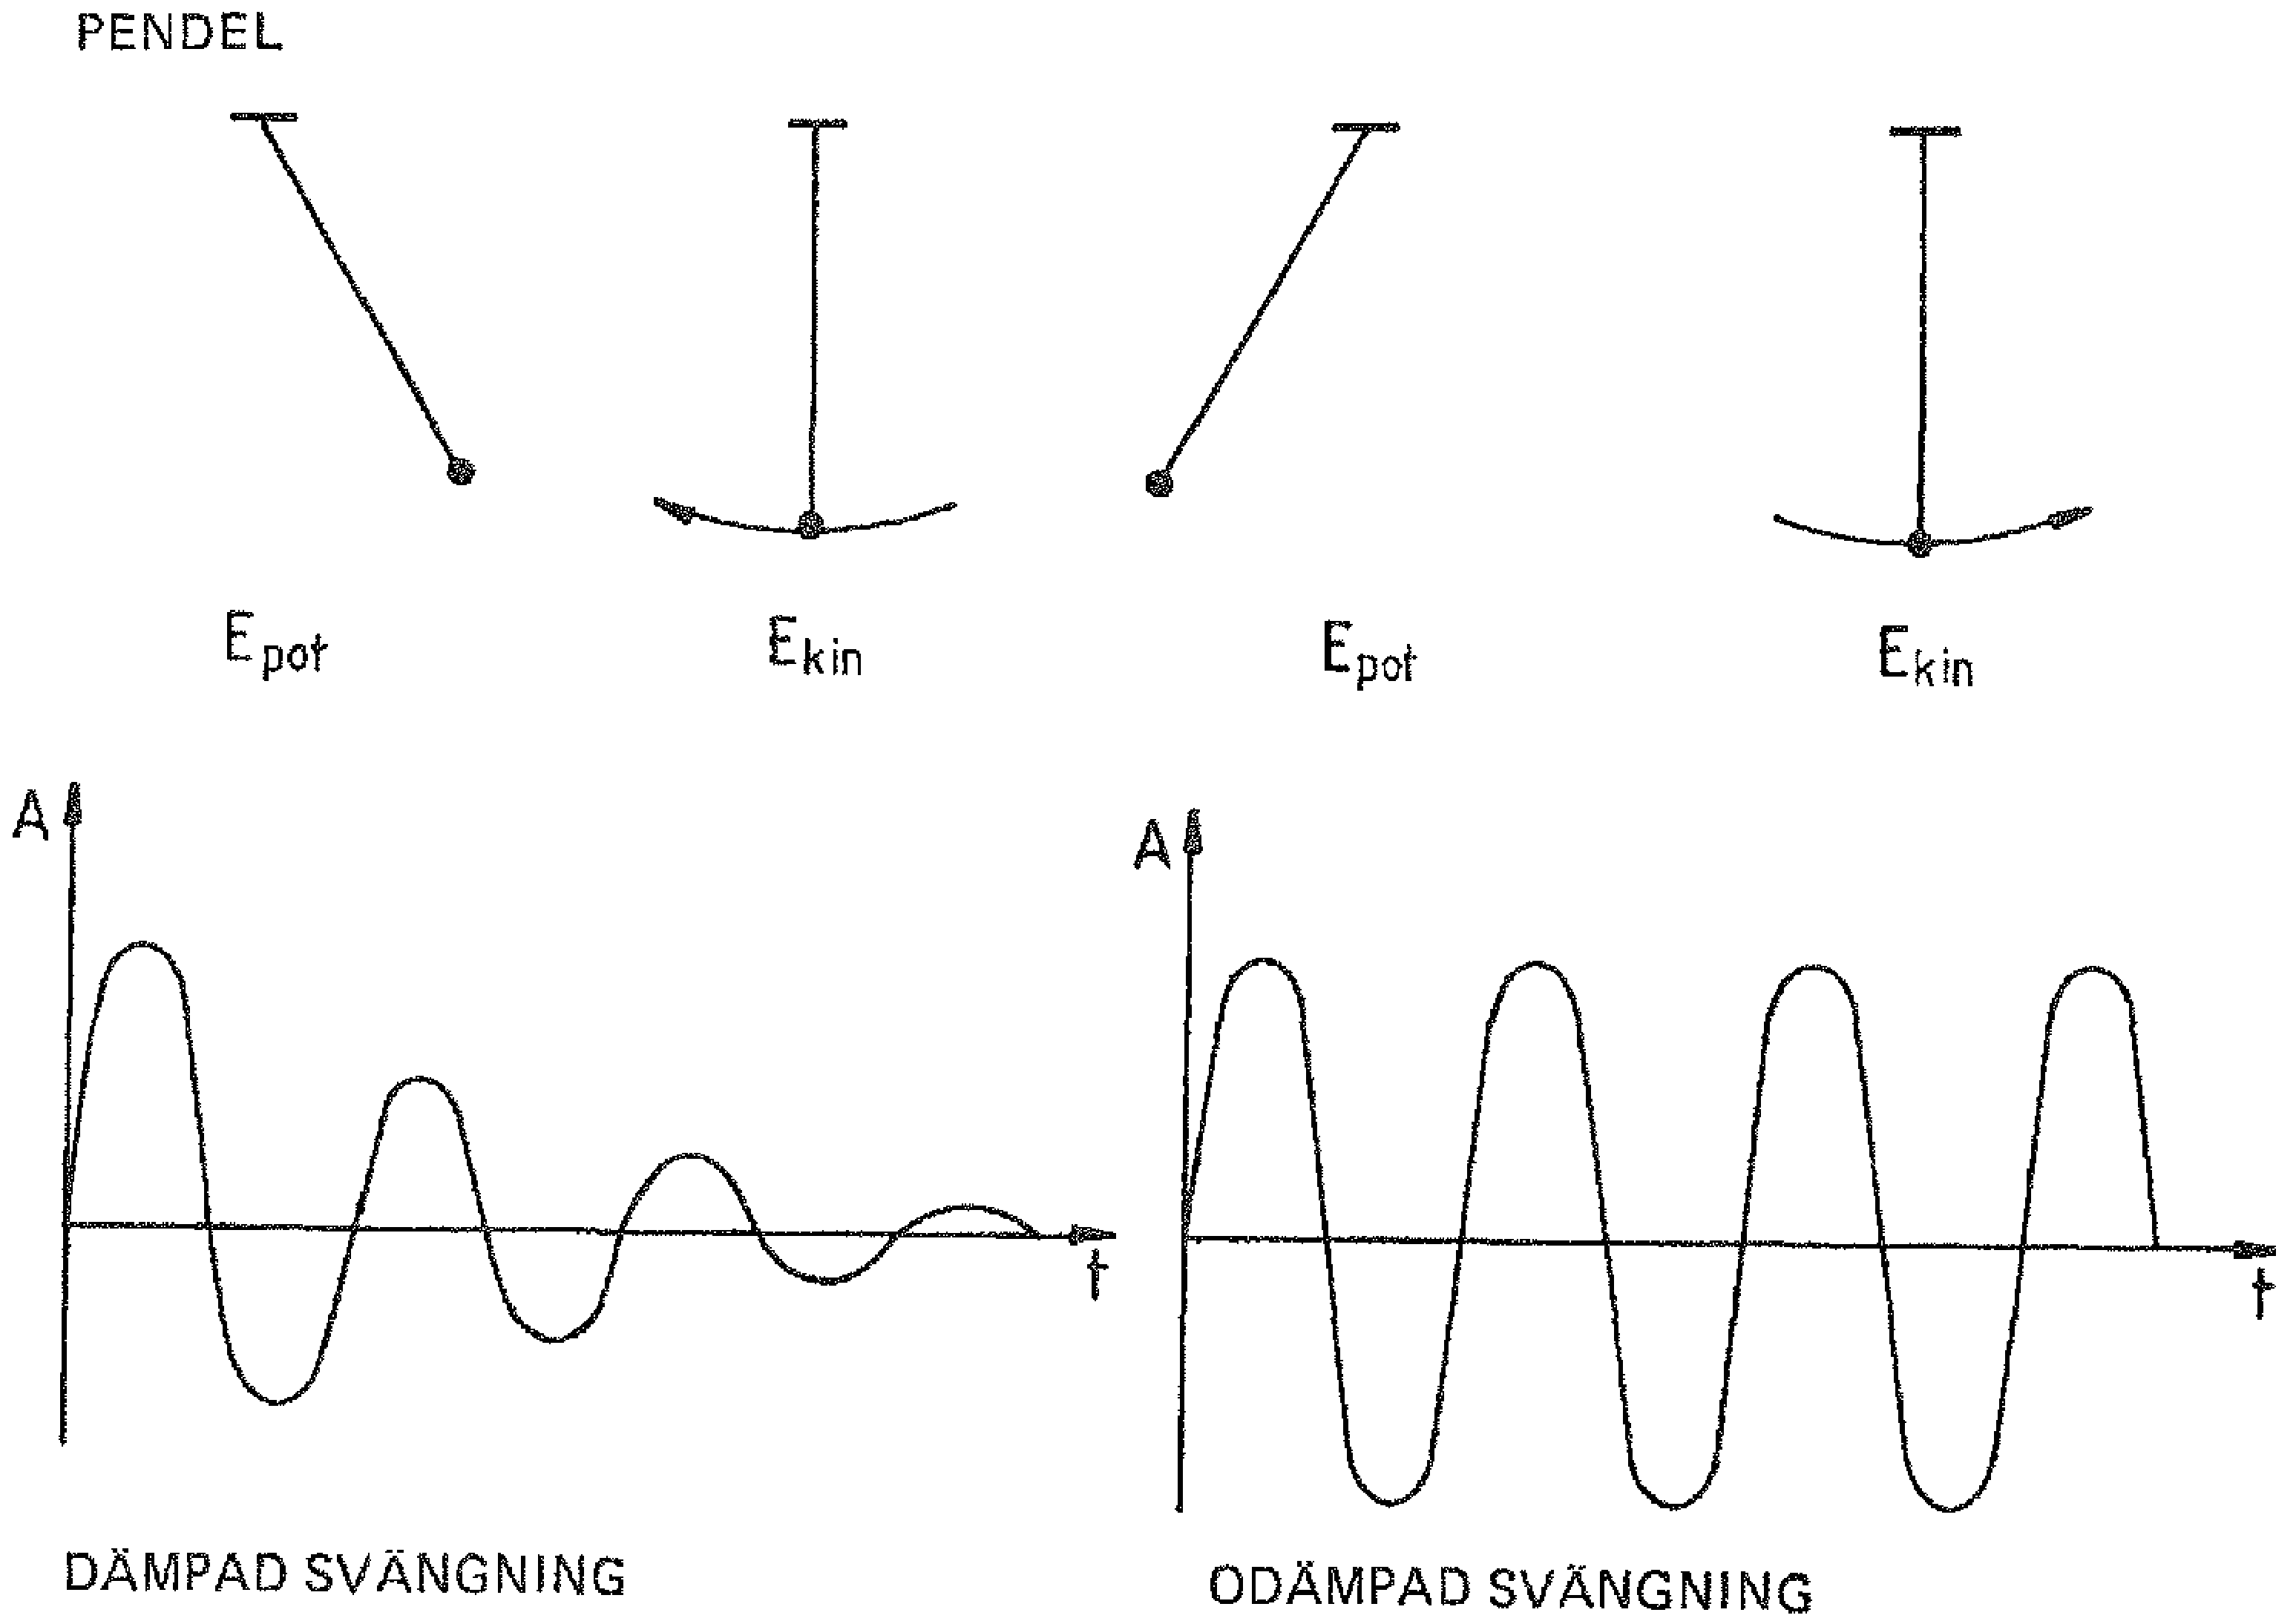
\includegraphics[width=\textwidth]{images/cropped_pdfs/bild_2_3-63.pdf}
\caption{Svängningar}
\label{fig:BildII3-63}
\end{figure}

\subsubsection{Dämpad svängning}
\index{dämpad~svängning}
Radiosändningar med telegrafi genomfördes i början av 1900-talet med dämpade
svängningar.
Det vill säga en svängning vars amplitud minskar tills svängningen upphört.

Svängningen skapades av en elektrisk gnista i ett gnistgap.
Gnistgapet kopplades till en avstämningskrets som gjorde att svängningsenergin
koncentrerades till en mer bestämd radiofrekvens.

De dämpade svängningarna orsakade på grund av den stora bandbredden störningar
som begränsade användbarheten för telegrafi.

\subsubsection{Odämpad svängning}
\index{odämpad~svängning}
\index{kontinuerlig~svängning}
\index{continuous~wave}
Begreppet odämpad svängning infördes för drygt 100 år sedan för att särskilja
en sinussvängning med konstant amplitud och frekvens från den dämpade
svängningen.

Till skillnad mot en dämpad svängning har en odämpad svängning en begränsad
bandbredd och går att använda för flera modulationsformer.
På engelska döptes svängningen till \emph{Continuous Wave} och förkortningen CW
används fortfarande av radioamatörer som en beteckning för telegrafi.

När fördelarna med odämpade sinusvågor blev tydliga och när oscillatorer med
radiorör blev tillgängliga runt år 1913 började myndigheter efter några år
införa begränsningar för användningen av gnistsändare.
Begränsningarna utökades genom internationella överenskommelser och under
1930-talet förbjöds användning av sändare med dämpade svängningar.

\subsection{LC-oscillatorer}
\textbf{HAREC a.\ref{HAREC.a.3.6.1}, a.\ref{HAREC.a.3.6.2}, a.\ref{HAREC.a.3.6.3}\label{myHAREC.a.3.6.1}\label{myHAREC.a.3.6.2}\label{myHAREC.a.3.6.3}}
\index{LC-oscillator}
\index{oscillator!LC}

\subsubsection{Variabel frekvens oscillator -- VFO}
\index{oscillator!VFO}
\index{oscillator!variabel frekvens}

\begin{wrapfigure}[32]{R}{0.5\textwidth}
  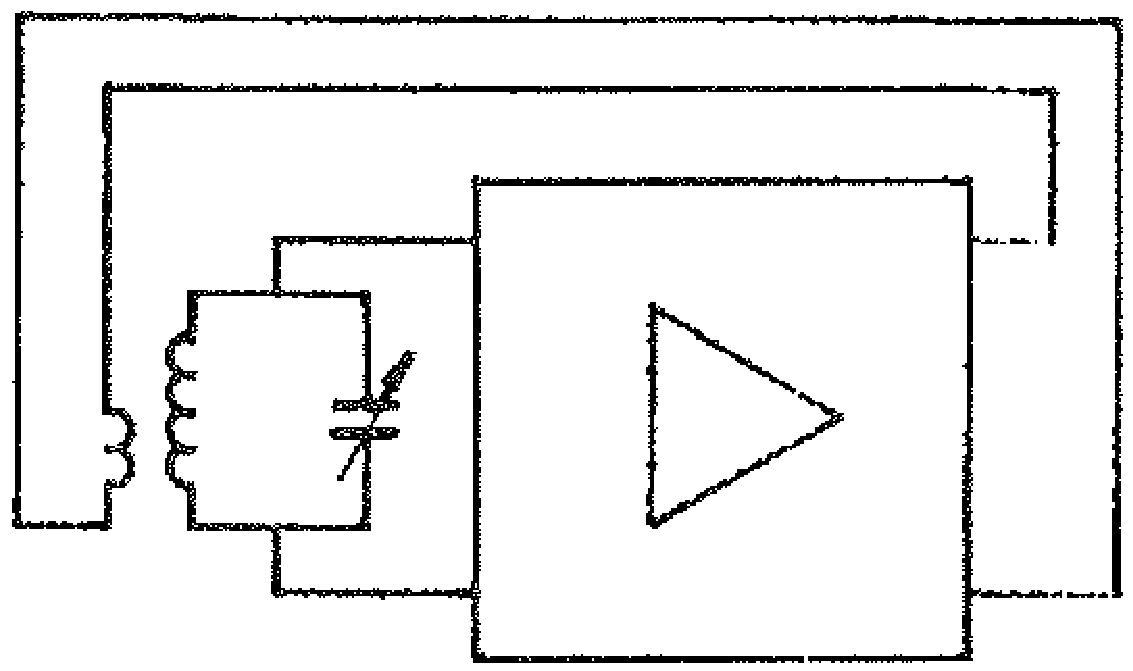
\includegraphics[width=0.5\textwidth]{images/cropped_pdfs/bild_2_3-66.pdf}
  \caption{Oscillator enligt Meissner}
  \label{fig:BildII3-66}

  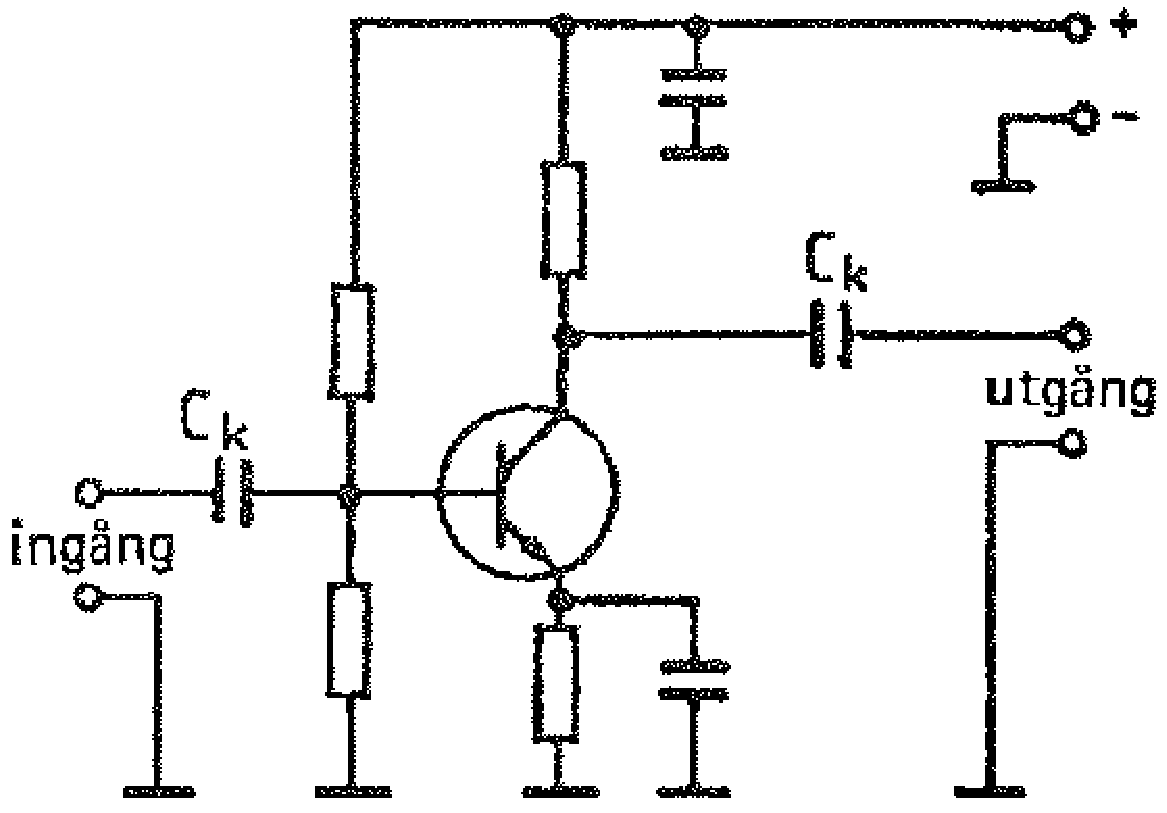
\includegraphics[width=0.5\textwidth]{images/cropped_pdfs/bild_2_3-67.pdf}
  \caption{Emitterkopplad förstärkare}
  \label{fig:BildII3-67}

  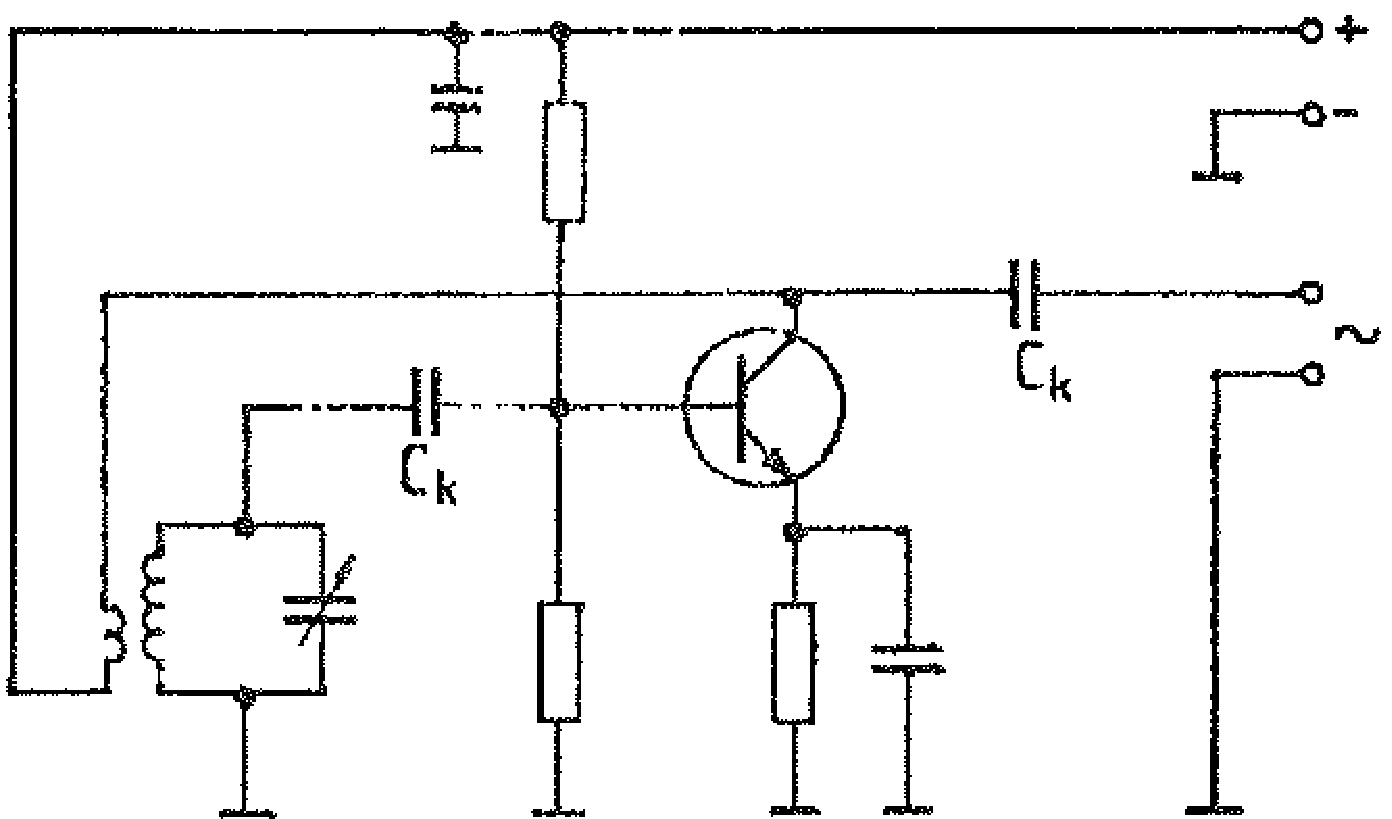
\includegraphics[width=0.5\textwidth]{images/cropped_pdfs/bild_2_3-68.pdf}
  \caption{Komplett Meissneroscillator}
  \label{fig:BildII3-68}
\end{wrapfigure}

En oscillator med inställbar frekvens kallas för VFO (variabel
frekvensoscillator).
Förutom frekvensstabilitet fordras också, att noggrann inställning och
avläsning av frekvensen ska kunna göras.

En LC-oscillator är urtypen för en oscillator med variabel frekvens.
Meissner-kopplingen är lätt att urskilja och används här för att beskriva
grundprincipen för en oscillator i stort.
Bl.a. Colpitts- och Clapp-kopplingarna har emellertid bättre stabilitet och
inställbarhet i återkopplingsledet

\subsubsection{Meissner-koppling}
\index{Meissner-koppling}
\index{oscillator!Meissner-koppling}

Bild \ref{fig:BildII3-66} visar en Meissner-oscillator, som består av en
LC-svängningskrets med återkopplingsspole och en förstärkare.
Magnetfältet mellan induktansen i svängningskretsen och återkopplingsspolen är
polariserat så att en förändring i utsignalen medverkar till självsvängning.
(Motsatsen är motkoppling.)

Förstärkaren kan till exempel vara en emitterkopplad transistorförstärkare enligt bild
\ref{fig:BildII3-67}.
Kopplingskondensatorerna \(C_k\) är nödvändiga för att förhindra kortslutning
av de likspänningar som bestämmer arbetspunkten för transistorn.
Å andra sidan kan växelspänningssignalerna passera till och från transistorn.

Återkopplingsvägen görs i detta fall så, att svängningskretsen kopplas
parallellt över förstärkaringången som visas i bild \ref{fig:BildII3-68}.
Återkopplingsspolen fungerar som förstärkarens kollektorresistor.

\subsection{Självsvängningsvillkoret}
\index{oscillator!självsvängningsvillkoret}

\begin{wrapfigure}{R}{0.5\textwidth}
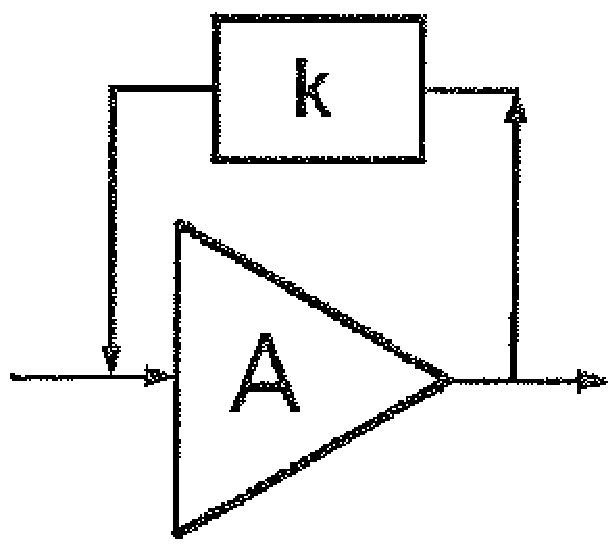
\includegraphics[width=0.5\textwidth]{images/cropped_pdfs/bild_2_3-69.pdf}
\caption{Svängningsvillkoret}
\label{fig:BildII3-69}
\end{wrapfigure}

Självsvängning i en förstärkare uppstår genom återkoppling, som visas i
bild \ref{fig:BildII3-69}.
Signalspänningen \(\hat{U}_{in}\) över ingången blir förstärkt med
faktorn \(A\).
När som i bild \ref{fig:BildII3-68} förstärkaren är emitterkopplad, blir
utsignalen fasvriden 180\degree~i förhållande till insignalen.
Fasvridningen \(\alpha=180\degree\) betecknas här med minustecken, alltså blir
förstärkningen \(-A\).

På förstärkarens utgång fås en signalspänning \(\hat{U}_{ut}\) med sambandet

\[\hat{U}_{ut} = -A \cdot \hat{U}_{in}\]

En del av utsignalen återförs (återkopplas) till ingången.
I en Meissner-oscillator sker återkopplingen med en induktor, som är
induktivt kopplad till svängningskretsens induktor.

Kvoten \(k\) mellan den återkopplade signalspänningen \(\hat{U}_{ut}\) och
signalspänningen out på förstärkarens utgång kallas återkopplingsfaktor.
Den återkopplade spänningen \(\hat{U}_k\) fasvrids så att den kommer
''i fas med'' med insignalen.
För den återkopplade signalen fås då sambandet

\[\hat{U}_k = -k \cdot \hat{U}_{ut}\]

Tillräcklig signalspänning från utgången måste återföras till ingången
för att det ska uppstå självsvängning.
Det sker när den återkopplade signalspänningen \(\hat{U}_k\) är minst lika stor
som ingångsspänningen \(\hat{U}_{in}\) och är i rätt fasläge, dvs. i
detta exempel

\[
\hat{U}_k \geq \hat{U}_{in}
\quad \text{eller} \quad
-k \cdot \frac{\hat{U}_{ut}}{A}
\quad \text{eller} \quad
k \geq \frac{1}{A}
\]

Självsvängningsvillkoret blir

\[
k \geq \frac{1}{A}
\quad \text{eller} \quad
k \cdot A \geq 1
\]

Ett \(k \cdot A \approx 3\) är önskvärt för att oscillatorn ska svänga igång
snabbt.

\subsubsection{Hartley-koppling}
\index{Hartley-koppling}
\index{oscillator!Hartley-koppling}
\index{Huth-Kügn-koppling}
\index{oscillator!Huth-Kügn-koppling}
\index{Tuned Grid Tuned Plate-koppling}
\index{oscillator!Tuned Grid Tuned Plate-koppling}

\begin{wrapfigure}[25]{R}{0.5\textwidth}
  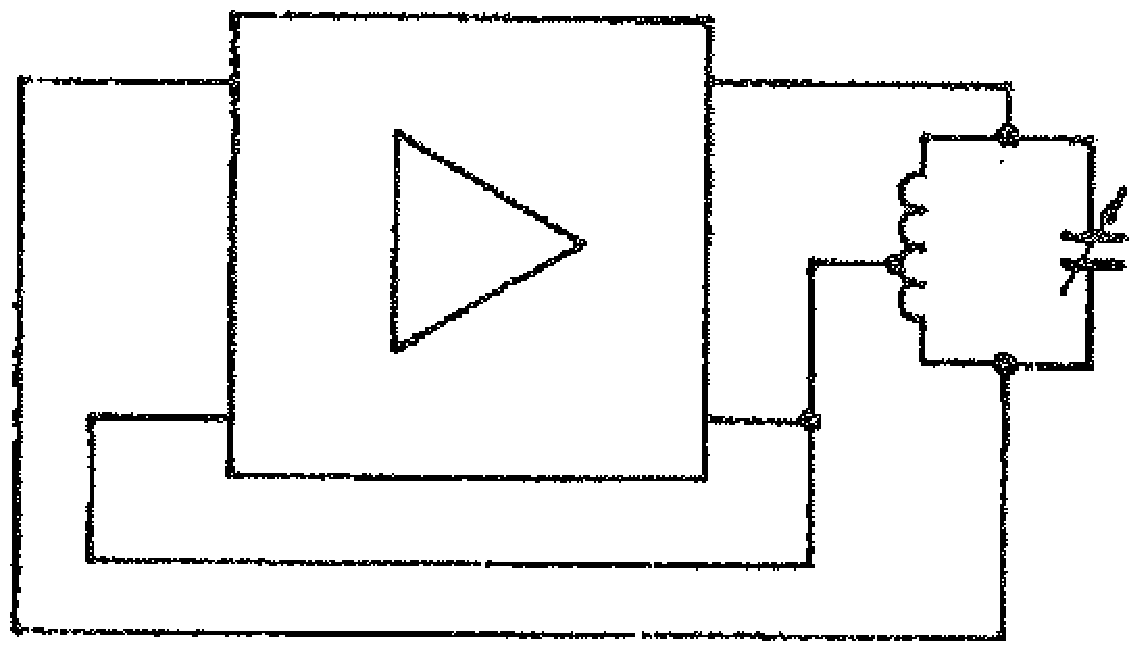
\includegraphics[width=0.5\textwidth]{images/cropped_pdfs/bild_2_3-70.pdf}
  \caption{Hartley-koppling}
  \label{fig:BildII3-70}

  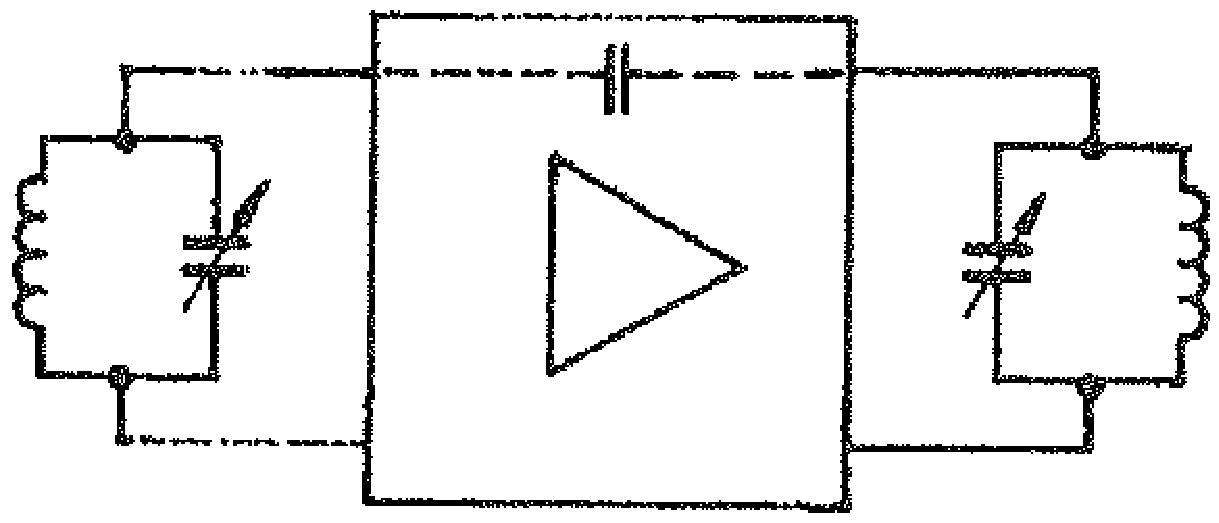
\includegraphics[width=0.5\textwidth]{images/cropped_pdfs/bild_2_3-71.pdf}
  \caption{TPTG-koppling}
  \label{fig:BildII3-71}

  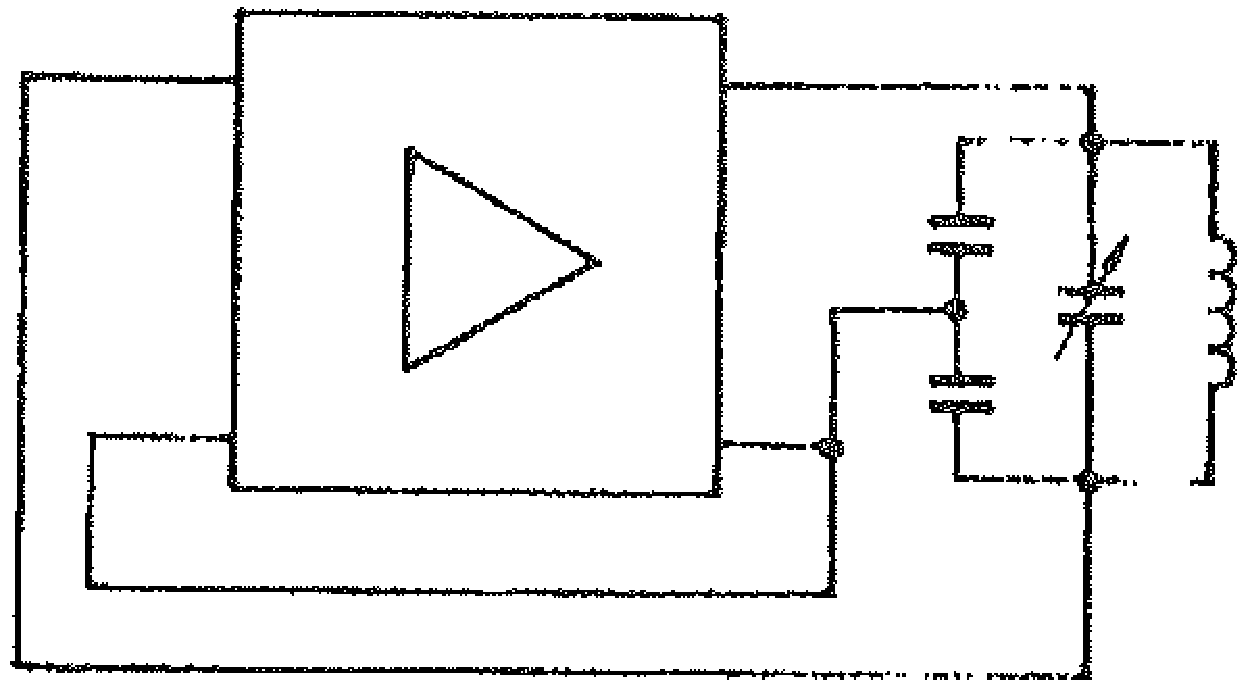
\includegraphics[width=0.5\textwidth]{images/cropped_pdfs/bild_2_3-72.pdf}
  \caption{Colpitts-koppling}
  \label{fig:BildII3-72}
\end{wrapfigure}

Bild \ref{fig:BildII3-70} visar en Harley-koppling.

Återkopplingen sker galvaniskt över ett uttag på induktorn i oscillatorns
LC-krets.

Bild \ref{fig:BildII3-71} visar en Huth-Kühn eller TGTP-koppling
(tuned grid -- tuned plate)

Kopplingen är en förstärkare med LC-kretsar både på in- och utgång.
Båda kretsarna är avstämda till samma frekvens.
Återkopplingen sker över de inre kapacitanserna mellan elektronrörets elektroder
resp. mellan transistorns materialskikt.
Denna koppling är av flera skäl inte särskilt vanlig.

\subsubsection{Colpitts-koppling}
\index{Colpitt-koppling}
\index{oscillator!Colpitt-koppling}

Bild \ref{fig:BildII3-72} visar en Colpitt-koppling.

Återkopplingen sker över en kapacitiv spänningsdelare, som ingår som
en del av oscillatorns LC-krets.

\subsubsection{Clapp-koppling}
\index{Clapp-koppling}
\index{oscillator!Clapp-koppling}

Denna koppling är en variant av Colpitts-kopplingen.
Vridkondensatorn för frekvensinställningen är seriekopplad med spänningsdelarens
kondensatorer.
Clapp-oscillatorns frekvensstabilitet är god.

Vi utvecklar denna beskrivning vidare med bild \ref{fig:BildII3-73a}.
Vridkondensatorn samt en fast och en trimningsbar kondensator är kopplade
parallellt med varandra.
Alla tre kondensatorerna är i sin tur seriekopplade med den kapacitiva
spänningsdelaren \(C_3/C_4\).
Förstärkarens ingång är kopplad till den övre anslutningen av \(C_3\).
Utgången från oscillatorns förstärkare återkopplas över dämpresistorn
\(R_{ct}\) till mitten av spänningsdelaren \(C_3/C_4\)
(återkopplingskretsen).

Bild \ref{fig:BildII3-73b} visar förstärkaren i en Clapp-koppling.
Förstärkarens arbetspunkt bestäms av spänningsdelaren \(R_1/R_2\).
Ingen kopplingskondensator behövs eftersom det enbart finns kondensatorer
mellan förstärkaringång och jord.
Kondensatorn \(C_6\) avkopplar kollektorn på transistor \(T_1\) HF-mässigt till
jord.
Förstärkaren är alltså kollektorkopplad.

Kondensatorn \(C_7\) kopplar oscillatorns utsignal till buffertsteget.
För frekvensstabilitetens skull stabiliseras spänningen 8~V med en
LC-krets som avkopplas HF-mässigt med en kondensator.

\subsection{Frekvensinställning och bandspridning}
\index{oscillator!frekvensinställning}
\index{oscillator!bandspridning}

\begin{wrapfigure}{R}{0.5\textwidth}
  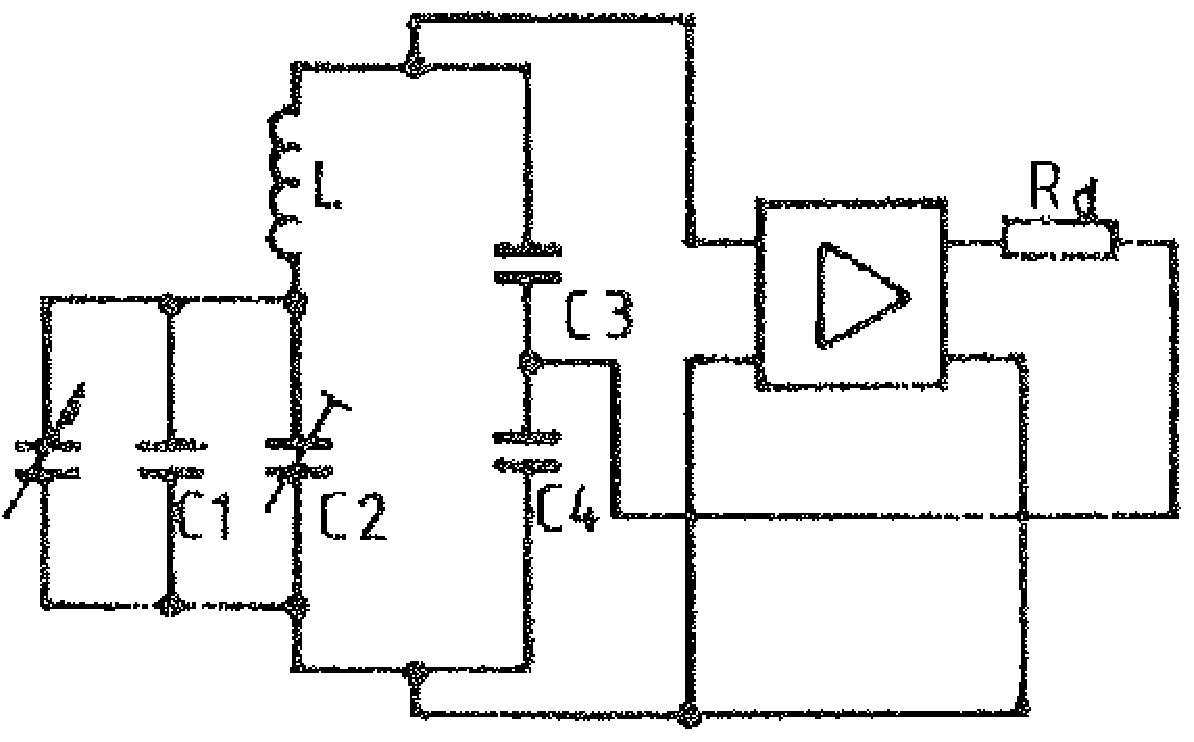
\includegraphics[width=0.5\textwidth]{images/cropped_pdfs/bild_2_3-73a.pdf}
  \caption{Clapp-koppling}
  \label{fig:BildII3-73a}

  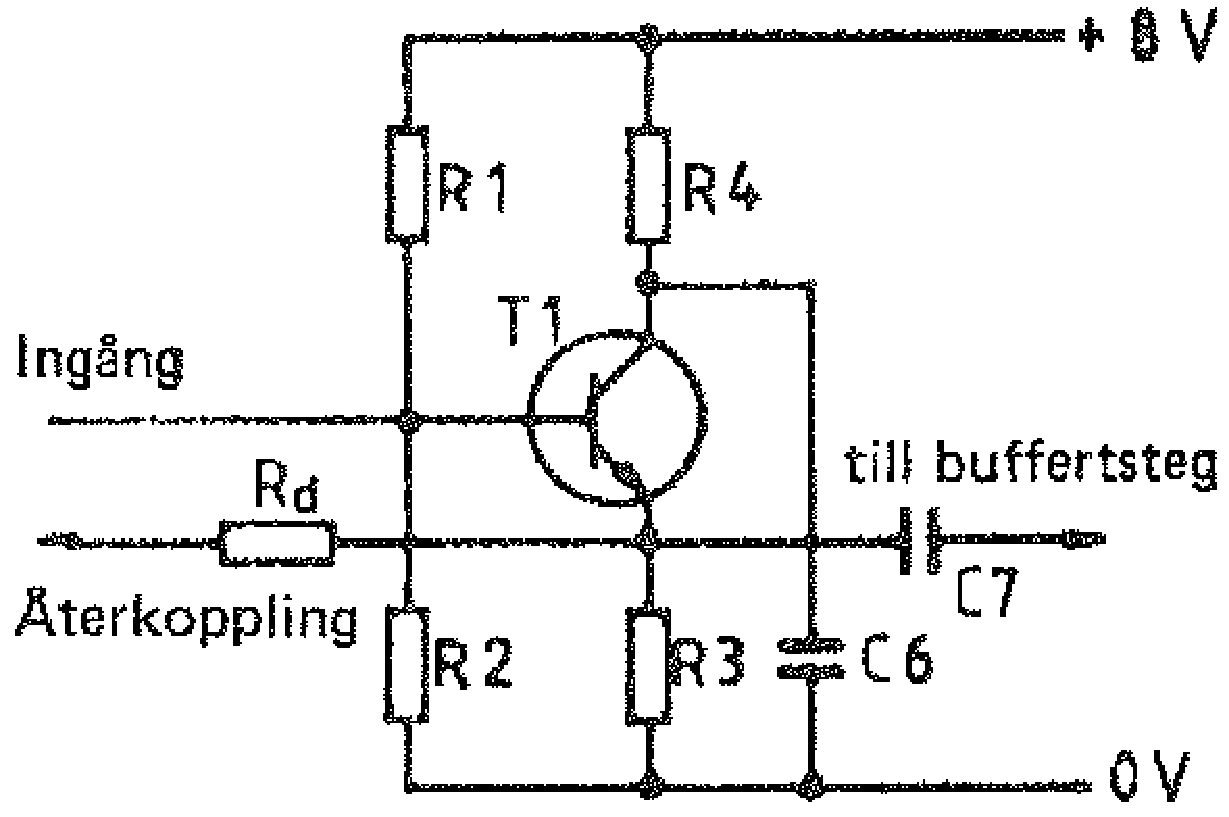
\includegraphics[width=0.5\textwidth]{images/cropped_pdfs/bild_2_3-73b.pdf}
  \caption{Förstärkare i Clappkoppling}
  \label{fig:BildII3-73b}

  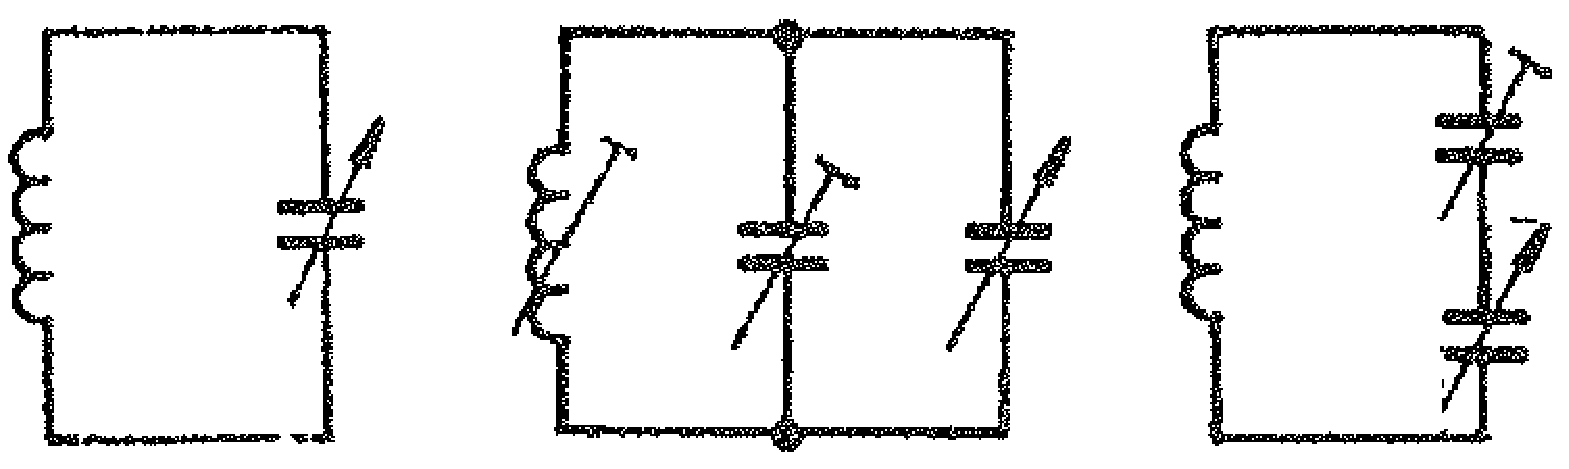
\includegraphics[width=0.5\textwidth]{images/cropped_pdfs/bild_2_3-74.pdf}
  \caption{Bandspridning}
  \label{fig:BildII3-74}
\end{wrapfigure}

Bild \ref{fig:BildII3-74} illustrerar stegvis hur man åstaokommer
bandspridning.
Att ställa in frekvensen i en LC-oscillator gjordes förr oftast med en
vridkondensator.
I moderna mottagare och sändare används i stället en så kallad varicap, som
styrs med en likspänning.

Med en svängningskrets med endast en induktor och en vridkondensator, skulle
alla amatörradiobanden endast vara smala områden utspridda på en mekanisk
skala, dvs. över vridkondensatorns hela kapacitansområde, varvid
kapacitansen kan varieras med förhållandet 1:5 à 1:10, till exempel
10-50~pF à 10-100~pF.

För att i stället få vart och ett av amatörradiobanden utspridda över större
delen av skalan kan man ordna med bandomkoppling och så kallad bandspridning.
Man parallellkopplar då en relativt stor fast kapacitans med vridkondensatorns
relativt lilla kapacitans.
Den totala kapacitansvariationen i LC-kretsen blir då liten, trots att
kondensatorns hela kapacitansområde utnyttjas.
Resultatet blir en frekvensskala med större upplösning, det vill säga bättre
avläsningsnoggrannhet.

Bandspridning kan också ordnas med två seriekopplade kondensatorer,
varav den större görs variabel.
Typiskt värde på vridkondensatorn i en kortvågsutrustning är då 100--500~pF
och den fasta kondensatorn mycket mindre än så.
